\include{MeijeCours}

\newboolean{versionprof}  % Cette variable booléenne permet le contrôle de la compilation selon la version professeur (avec les preuves, commentaires pédagogiques etc...) si true ou selon la version élève (de ''base'') si false.
\setboolean{versionprof}{false}

% =============================================================================================
%                                                                                      Début du texte 
% =============================================================================================

\author{Spé NSI - Lycée du parc}  % Pour spécifier l'auteur qui sera affiché sous le titre
\title{Représentation approximative des nombres réels : \\ {les nombres flottants}}  % Titre 
\date{Année 2020 - 2021} %en utilisant \today on obtiendra la date courante lors de la production du document
\renewcommand{\thesection}{\Roman{section}}  % permet de numéroter les sections en chiffres romains
\pagestyle{fancy}

\lhead{NSI}   %  Indiquer la classe ici  
\rhead{Approximation des réels par les flottants}		% Indiquer la date pour rendre le devoir ici


\fancyfoot[C]{\thepage} % bas de page : centre par exemple:  - \thepage\ -
\fancyfoot[L]{} % bas de page : gauche
\fancyfoot[R]{} % bas de page : droite
\newcommand{\p}[1]{ \left( #1 \right)}   %parenthèse
\newcommand\abs[1]{|{#1}|}
\newcommand{\intent}[2]{[\![ #1 , #2 ]\!]} %intervalle fermé entier
\newcommand{\pe}[1]{ \left\lfloor #1 \right\rfloor} %partie entière crochets bas
\begin{document}
\maketitle  %produit le titre conformément aux instructions données par \author, \date ...etc
\vspace{0.2cm}
\maketitle  %produit le titre conformément aux instructions données par \author, \date ...etc
\thispagestyle{empty}
% ------------------------------------------------   Introduction   -------------------------------------------

\renewcommand{\abstractname}{Introduction\hfill}
\begin{abstract} 
Il est tout simplement impossible de représenter de manière exacte les nombres réels dans la mémoire d'un ordinateur. Les nombres flottants en constituent l'approximation usuellement utilisée, par exemple pour les calculs scientifiques.
\end{abstract}    
\vskip 1cm

\section{\'Ecriture scientifique}

\exercice{}

\begin{enumerate}[1.]
  \item Rappeler le principe de l'écriture scientifique des nombres utilisée en sciences physique.
  \item \'Ecrire les nombres suivants sous forme scientifique : 
  
  \begin{center}
a = 2021\hskip 0.5cm b = 0,0000005468 \hskip 0.5cm c = -897164,236  \hskip 0.5cm d = -897164,236 , \hskip 0.5cm e = -4,236 
\end{center}
  \item On donne $x = 11,25 \times 10^{125}$ et $y = 2,6\times 10^{-84}$. Que dire de $x+y$ ?
\end{enumerate}
\lignes{10}

Pour comprendre, la représentation approximative des réels par les flottants, on étudie la situation simplifiée et plus familière des nombres en notation scientifique. On la reproduit à l'aide de trois éléments : un signe, une mantisse qui est un nombre décimal et un exposant : 

\begin{center}
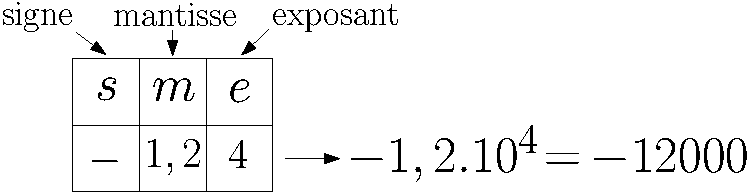
\includegraphics[width=10cm]{repr-nbs-2.pdf}
\end{center}

Mais il faut fixer une taille limitée pour la mantisse et l'exposant afin de pouvoir les coder.
\medskip

Si l'on suppose que la mantisse est codée sur $t+1$ chiffres (décimaux) et que l'exposant est un entier entre $e_{\min}$ et $e_{\max}$ on peut alors représenter tous les décimaux de la forme 
$$ \pm \p{c_0 + \frac{c_1}{10} + \dots + \frac{c_t}{10^t}} 10^e$$

avec $e \in \intent{e_{\min}}{e_{\max}}$ et chaque chiffre $c_i \in \intent{0}{9}$ avec $c_0 \neq 0$ (excepté pour le nombre $0$ où l'on ne peut pas imposer $c_0 \neq 0$. Le nombre $0$ a un traitement particulier). 

\exercice{}

Si l'on prend $e_{\min}=-1$, $e_{\max}=1$ et $t=1$ alors on peut représenter les décimaux de la forme 
$$ \pm \p{c_0 + \frac{c_1}{10}} 10^{-1} \qquad \pm \p{c_0 + \frac{c_1}{10}} 10^{0} \qquad \pm \p{c_0 + \frac{c_1}{10}} 10^{1}$$


Quel est alors
\medskip

\begin{enumerate}
\item le plus grand nombre représentable ?\\

\item le plus petit ?\\

\item le plus petit strictement positif ?\\

\item le plus petit nombre après $1$ ?\\

\item Combien de nombres différents sont représentable ?

\end{enumerate}

\lignes{4}

\begin{center}
------------------------------
\end{center}

Dans le cas où $t=0$, $e_{\min}=-1$ et $e_{\max}=1$, les nombres décimaux représentables sont :
\medskip

-90, -80, -70, -60, -50, -40, -30, -20, -10, -9, -8, -7, -6, -5, -4, -3, -2, -1, 
-0.9, -0.8, -0.7, -0.6, -0.5, -0.4, -0.3, -0.2, -0.1, 0, 0.1, 0.2, 0.3, 0.4, 0.5, 
0.6, 0.7, 0.8, 0.9, 1, 2, 3, 4, 5, 6, 7, 8, 9, 10, 20, 30, 40, 50, 60, 70, 80, 90

\begin{center}

\includegraphics[width=18cm]{Representables3.pdf} % Image
\end{center}


Il est important de constater que l'écart entre deux grands nombres représentables est bien plus grand que celui entre deux nombres proches de $0$ : \begin{center}
{\bf  La répartition des décimaux représentables n'est pas uniforme\footnote{Il en sera de même pour les flottants.}}.


\end{center}
\vfill
\eject
\section{Norme IEEE 754}

\exercice{}

L'écriture binaire des entiers a été vue vu dans le chapitre sur la représentation des nombres.

\begin{enumerate}
  \item Quelle est la \og valeur\fg \ du premier chiffre (tout à droite) ?
  
  \item Quelles sont les valeurs des chiffres suivants vers la gauche ?
  
  \item Que représente en décimal le nombre $\overline{101001}^{(2)}$ ?
  
  \item On peut écrire de la même manière des nombres avec une virgule. Quelle est alors la valeur du premier chiffre après la virgule ?
  
  \item Que représente en décimal le nombre $\overline{1,101}^{(2)}$ ?
\end{enumerate}

\lignes{12}

\exercice{}

\'Ecrire une fonction python \verb+ChaineBinDec(c)+ qui prend en entrée une chaîne de caractères \verb+c+ représentant un nombre à virgule écrit en binaire et qui renvoie le nombre flottant de valeur correspondante.

\begin{lstlisting}
>>> ChaineBinDec('1,101')
1.625
\end{lstlisting}
\lignes{10}

En décimal on est habitué à ce que certaines fractions simples aient une représentation illimitée : 

\begin{center}
$\frac{1}{3} =  0,\underbrace{33333333333333333333333333333333333333...}_{\text{une infinité de 3}}$
\end{center}

En binaire, le problème est simplement un peu plus fréquent. Ainsi, le nombre $\textstyle \frac 1{10}$ a une écriture binaire illimitée et il n'est donc pas représentable exactement en machine ! C'est ce qui explique le résultat :
\smallskip

\begin{lstlisting}
>>> 0.1*0.2
0.020000000000000004
\end{lstlisting}
\begin{center}
------------------------------
\end{center}

La norme IEEE 754 standardise la représentation des flottants. C'est la norme la plus couramment utilisé dans les ordinateurs. Elle se décline en deux versions : le format \emph{binary32} ou \emph{simple précision} utilise 32 bits pour représenter un flottant, 
le format \emph{binary64} ou \emph{double précision} utilise 64 bits pour représenter un flottant. Comme Python utilise le deuxième type sur nos machines, on va se concentrer sur celui-ci.
\medskip

Il y a principalement deux différences avec l'écriture scientifique : 
\smallskip

\begin{itemize}
  \item La mantisse est écrite en binaire, elle est donc dans l'intervalle $[1, 2[$
  \item l'exposant est un entier entre -1022 et 1023 qui est stocké de manière décalé d'une valeur $d = 1023$. On remarque que les 2048 valeurs représentables avec 11 bits ne sont pas toutes utilisées ; il \og manque\fg\ les valeurs $-1023$ et $1024$. 
\end{itemize}

\begin{center}
	\begin{tabular}{| c | c | c | }
		\hline
		signe & exposant & fraction \\ \hline
		\end{tabular}
	
	\vspace{-0.3cm}
		\begin{tabular}{ c  c  c  }
	
		$\underbrace{\phantom{signe}}_{\text{1 bit}}$ & $\underbrace{\phantom{exposant}}_{\text{11 bits}}$ & $\underbrace{\phantom{fraction}}_{\text{52 bit}}$ \\ 
	\end{tabular}
	
\end{center}


Si on note $s$ la valeur 0 (pour +) ou 1 (pour -) du signe, e la valeur de l'exposant et $m\in [1, 2[$ celui de la mantisse, la valeur du nombre représenté est :

\begin{center}
	$x = (-1)^s\times m\times 2^{e-d}$ 
\end{center}


Enfin une dernière difficulté ; le chiffre des unités de la mantisse étant toujours égal à 1, il n'est pas représenté, ainsi les 52 bits de la mantisse représente en fait la \emph{fraction} c'est à dire les bits de la partie fractionnaire de la mantisse.

On a donc : 
\begin{center}
		\begin{tabular}{| c || c | c | c | c | c || c | c | c | c | c | }
	\hline
	$s$ & $e_{10}$ & $e_9$ & $\dots$ & $e_1$  & $e_0$  & $f_1$ & $f_2$ & $\dots$ & $f_{51}$ & $f_{52}$  \\ \hline
\end{tabular}  

\end{center}

On a donc $e = \sum_{k=0}^{10} e_k 2^k$ et $m = 1+\sum_{n = 1}^{52}f_n 2^{-n} = 1 + f$


\exercice{}

Calculer le nombre représenté par la suite de bits : $\boxed{1} \boxed{10110100000}\boxed{011101100000\dots \, 0}$

\lignes{8}

\exercice{}

Déterminer les bits de la représentation du nombre x = 0,01203125

\lignes{8}

\exercice{}

\'Ecrire une fonction \verb+ChaineIEEE754(c)+ qui prend en entrée une chaîne de caractères
représentant les bits d'un nombre flottant en double précision et qui renvoie le nombre flottant de valeur correspondante.

\lignes{14}

{\bf \large Zéro et valeurs spéciales}
\bigskip

Tel que vu jusqu'à présent, le nombre 0 n'est pas représentable en IEEE 754. On utilise les valeurs de l'exposants qui restent libres : il y a deux zéro +0 avec s = 0, e = 0 et f = 0 et -0 avec s = 1, e = 0 et f = 0.

Il y a aussi deux infinis $+\infty$ avec s = 0, e = 2047 et f = 0 et $-\infty$ avec s = 1, e = 2047 et f = 0. Ils servent notamment à indiquer un dépassement de capacité.

Enfin on dispose aussi d'une valeur spéciale, notée {\bf NaN} (pour \emph{Not a Number}) qui représente les résultats d'opération invalides comme 0/0 ou $\sqrt{-1}$ avec s = 0, e = 2047 et f $not = 0$.

\end{document}


